% ================================== HEADER ====================================
\documentclass{article}           % Sets style/look of many things.
% \documentclass{report}          % part, chapters, front page etc.
\usepackage{exsheets}
\usepackage[utf8]{inputenc}       % Encoding of input files UTF-8
\usepackage[T1]{fontenc}
\usepackage[scaled]{beramono}     % Font
\usepackage{color}                % Color text
\usepackage{titlesec}             % Select alternative section titles
\usepackage{fancyvrb}
\usepackage{verbatim}             % Comment environment
\usepackage{listings}             % Format and render text/code etc.
\usepackage{minted}               % Much better syntax highlighting
\usepackage{float}                % Control of floating environment/figure
\usepackage{graphicx,  subfigure} % Better figures, graphics, units etc.
\usepackage{multicol}             % Multiple columns
\usepackage{amsmath}              % Math: Equation, split, align etc.
\usepackage{siunitx}              % SI units
\usepackage{mathtools}            % Different math tools to use with amsmath
\usepackage{amssymb}              % Math symbols
\usepackage[
    colorlinks,
    citecolor=black,              % I like links with standard black color
    filecolor=black,
    linkcolor=black,
    urlcolor=black
]{hyperref}                       % Links in TOC etc.
\usepackage[all]{hypcap}          % Better links to floating environment

\usepackage{tabto}
\newcommand\marginsymbol[1][0pt]{%
  \tabto*{0cm}\makebox[\dimexpr-1cm-#1\relax][r]{$\mathbb{P}$}\tabto*{\TabPrevPos}}

\renewcommand{\thesubsection}{\thesection.\alph{subsection}}
\title{\vspace{-2cm}INF3490/INF4490 Exercises - Week 5}
\author{Ole Herman S. Elgesem, Magnus Olden, Stian Petlund}
\date{\today}

% Removing paragraph indents is sometimes useful:
\setlength\parindent{0pt}

% Make margins smaller to fit more figures, tables etc on page: (optional)
\addtolength{\oddsidemargin}{-1.0in}
\addtolength{\evensidemargin}{-1.0in}
\addtolength{\textwidth}{2.0in}
\addtolength{\topmargin}{-0.8in}
\addtolength{\textheight}{1.6in}
% ==============================================================================

% ================================= DOCUMENT ===================================
\begin{document}
    \renewcommand\marginsymbol[1][0pt]{%
  \tabto*{0cm}\makebox[-1cm][c]{$\mathbb{P}$}\tabto*{\TabPrevPos}}

\maketitle
\(\mathbb{P}\) marks the programming exercises, we strongly recommend using
the python programming language for these. Exercises may be added/changed
after publishing.

\section{Single Layer Perceptron}
\subsection{}
In the perceptron below, what will the output be when the input is (0, 0)?
What about inputs (0, 1), (1, 1) and (1, 0)?
What if we change the bias weight to -0.5?

\begin{figure}[H]
\begin{center}
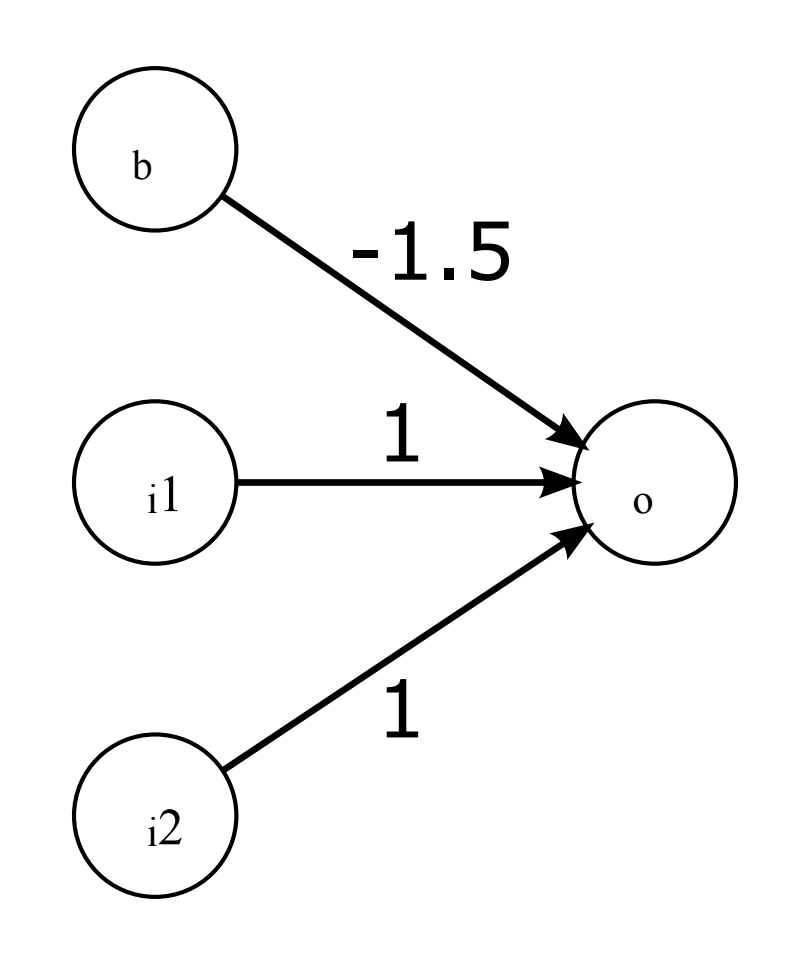
\includegraphics[width=0.3\textwidth]{fig1.png}
\caption{An illustrated example of a single layer perceptron}
\label{fig:slp}
\end{center}
\end{figure}

\subsection{}
Starting with random weights, how do you proceed in order to train the
perceptron above to perform any given binary operation?
\subsection{\marginsymbol}
Implement the perceptron, and train it to perform the logical functions NOT
(use only one of the inputs), NAND, and NOR. What happens when you try to
train it do the XOR function?

\section{Multi Layer Perceptron (MLP)}
The figure below shows a multilayer perceptron that constructs the XOR function.
How would you rewrite it to construct the binary equivalence function
(i.e. the output is above threshold when both inputs are either 0 or 1)? Can
you construct it so that it will detect equivalence for any combination of integer
inputs?

\begin{figure}[H]
\begin{center}
\includegraphics[width=0.6\textwidth]{fig21212.png}
\caption{An illustrated example of a multi layer perceptron}
\label{fig:mlp}
\end{center}
\end{figure}

\section*{Corrections and suggestions}
Corrections of grammar, language, notation or suggestions for improving these exercises are appreciated.
E-mail me at: \href{mailto:olehelg@uio.no}{\textbf{olehelg@uio.no}} or use
\href{https://github.com/olehermanse/INF3490-AI_Machine_Learning}{\textbf{GitHub}}
to submit an issue or create a pull request.
\end{document}
% ==============================================================================
